
%(BEGIN_QUESTION)
% Copyright 2013, Tony R. Kuphaldt, released under the Creative Commons Attribution License (v 1.0)
% This means you may do almost anything with this work of mine, so long as you give me proper credit

A FOUNDATION Fieldbus pressure transmitter is used as part of a {\it hydraulic load cell} system to measure the weight applied to a platform scale: the platform's weight presses against a piston, which exerts pressure in a hydraulic fluid according to the force/pressure/area formula $F = PA$.  The transmitter then senses this fluid pressure as a representative proportion of platform weight:

$$\includegraphics[width=15.5cm]{i03385x01.eps}$$

Assuming the circular piston has a diameter of 4 inches, determine the proper {\tt XD\_Scale}, {\tt OUT\_Scale}, and {\tt L\_Type} parameter values to make the transmitter functional over a platform weight range of 0 to 25,000 pounds.

\underbar{file i03385}
%(END_QUESTION)





%(BEGIN_ANSWER)

{\tt XD\_Scale} = 0 to 1989.4 PSI

\vskip 10pt

{\tt OUT\_Scale} = 0 to 25,000 pounds

\vskip 10pt

{\tt L\_Type} = Indirect

%(END_ANSWER)





%(BEGIN_NOTES)


%INDEX% Fieldbus, instrument ranging: setting XD_Scale and OUT_Scale parameters for an application

%(END_NOTES)


